\chapter{Verwandte Arbeiten}
\label{kap3}

Dieses Kapitel stellt weitere Arbeiten dar, die sich mit dem Thema der Laufplanung von sechsbeinigen Laufrobotern mittels Random Sampling auseinandergesetzt haben.

\section{Globaler Laufplaner nach André Herms}

Andrè Herms \autocite{herms2004} vergleicht zunächst die folgenden Algorithmen zur Laufplanung:
\begin{itemize}
  \item Random Sampling
  \item Greedy Verfahren
  \item Branch and Bound
  \item Lokale Suche
  \item Tabu-Suche
  \item Simulated Annealing
  \item Genetische Algorithmen
\end{itemize}

Dabei nutzt Herms die folgenden Kriterien:
\begin{itemize}
  \item Parallelisierbarkeit
  \item Speicherbedarf
  \item Anytime-Fähigkeit
  \item Allgemeine Anwendbarkeit
\end{itemize}

Es stellt sich heraus, dass nur die Algorithmen \emph{Random Sampling}, \emph{Lokale Suche} und \emph{Simulated Annealing} alle Kriterien mindestens erfüllen. Nach der Implementierung und erster Tests stellt sich heraus, dass das Random Sampling die Kriterien am besten erfüllt, da die Lokale Suche sowie das Simulated Annealing die Lösungen zu langsam erstellen. \autoref{Kap3:BewertungRandomSampling} bewertet das Random Sampling anhand der genannten Kriterien. Auch hier wird nochmals deutlich, dass das Random Sampling positiv abschneidet.

\begin{table}[!t]
  \caption{Bewertung des Random Samplings}
  \label{Kap3:BewertungRandomSampling}
  \renewcommand{\arraystretch}{1.2}
  \centering
  \sffamily
  \begin{footnotesize}
    \begin{tabularx}{0.9\textwidth}{l X}
      \toprule
      \textbf{Kriterium} & \textbf{Erfüllung}\\
      \midrule
      \emph{Parallelisierbarkeit} & Lösungen können ohne großen Aufwand unabhängig voneinander generiert werden. Am Ende müssen diese nur noch synchronisiert werden, so dass die Lösung mit der besten Bewertung übernommen wird.\\
      \addlinespace
      \emph{Speicherbedarf} & Der Algorithmus benötigt kaum Speicher, da immer nur eine Lösung generiert wird und diese die vorherige beste Lösung überschreibt.\\
      \addlinespace
      \emph{Anytime} & Das Kriterium ist erfüllt, sobald eine Lösung generiert ist. Allerdings kann es passieren, dass in einer bestimmten Zeit noch keine gute Lösung vorhanden ist.\\
      \addlinespace
      \emph{Anwendbarkeit} & Der Algorithmus lässt sich auf jedes Problem der Laufplanung anwenden. Die Qualität hängt allerdings vom Anteil guter Lösungen, die im Lösungsraum vorhanden sind. Außerdem spielt die konkrete Implementierung des Algorithmus eine große Rolle. Insgesamt gilt, dass je länger der Algorithmus läuft, desto besser sind potentiell die Lösungen.\\
      \bottomrule
    \end{tabularx}
  \end{footnotesize}
  \rmfamily
\end{table}

Daher entscheidet die Arbeit von André Herms, dass das Random Sampling für den Laufplaner genutzt werden soll, da es zwischen allen Algorithmen am besten abschneidet.

Der von André Herms daraufhin entwickelte Laufplaner für den \emph{Lauron III} basiert auf der 3D-Bibliothek OpenInventor \autocite{inventor}. Dieses Toolkit basiert wiederum auf OpenGL und ist in C++ implementiert. Des Weiteren ist es objektorientiert implementiert. Auf Grund dieser Tatsache existieren Klassen bzw. Objekte, die nun beschrieben werden:
\begin{itemize}
  \item \emph{World}: speichert die Objekte der Sicht auf die Landschaft und den Roboter. 
  \item \emph{Terrain}: enthält die Informationen über die Höhenkarte.
  \item \emph{Eyes}: stellt die Sicht auf die Landschaft dar.
  \item \emph{Robot}: ist verantwortlich für die Robotersteuerung und definiert außerdem die inneren Objekte \emph{Head} und \emph{Leg}.
\end{itemize}  
  
\begin{figure}[t!]
  \centering
  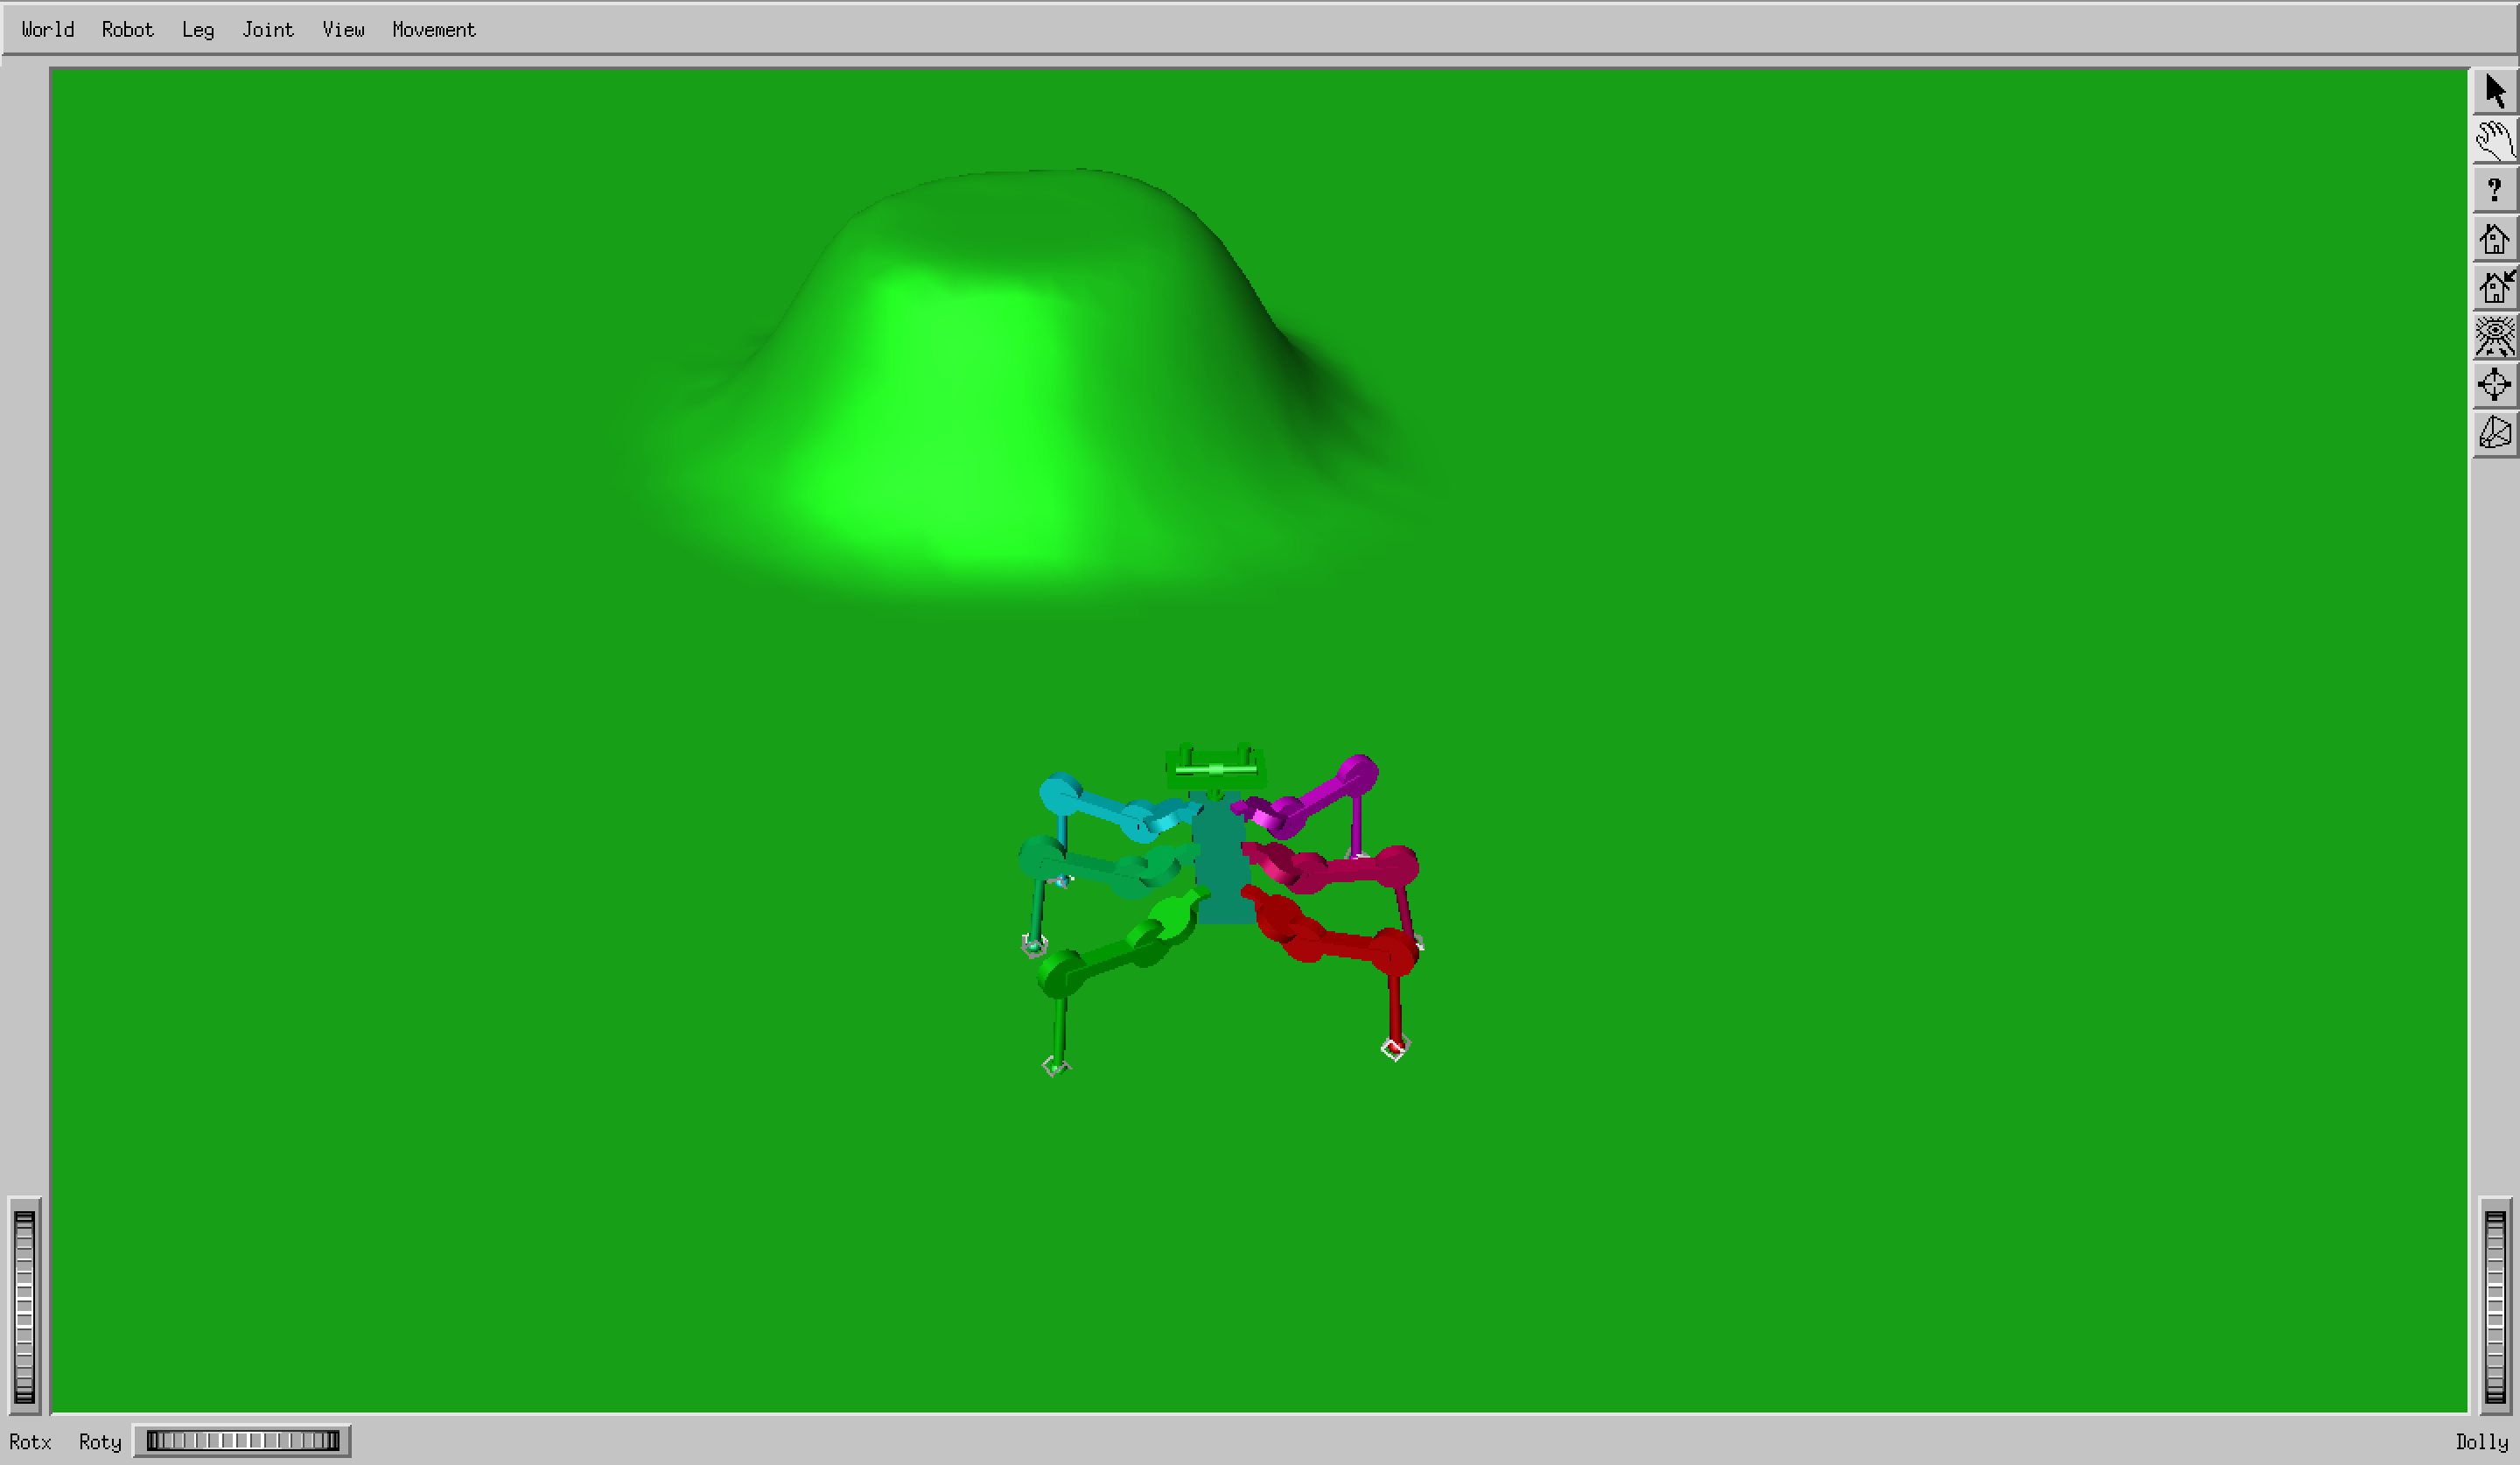
\includegraphics[height=8cm]{kapitel3/openinventor-lauron}
  \caption{Screenshot aus der OpenInventor-Umgebung}
  \label{Kap4:OpenInventorLauron}
\end{figure}

Für jedes dieser Darstellungsobjekt in OpenInventor wird ein \emph{SoSeperator} benötigt. Da der Name dieses Objekts einzigartig sein muss, sind die Objekte auch nur einmalig nutzbar. Dies erschwert die Aufgabe, später einmal mehrere Roboter gleichzeitig in der Simulation zu testen. Code-technisch sollte das dem Design-Pattern \emph{Singleton} folgen. Der Laufplaner sichert diese allerdings nicht derart ab.

Des Weiteren stellt das Terrain-Objekt die Höhenkarte der Landschaft in OpenInventor zur Verfügung. Dies entspricht nicht dem, was dem Roboter tatsächlich an Kartenmaterial zur Verfügung hat.

Eine Konfigurationsdatei existiert bereits in dieser Umgebung, die es ermöglichen soll, auch andere Robotermodelle zu testen. Diese wird für den Laufalgorithmus allerdings nicht genutzt, da dort Roboterangaben direkt im Quelltext definiert sind.

Weiterhin wird die aktuelle Fußkonfiguration sowie die Fußposition getrennt voneinander gespeichert. Die Fußkonfiguration ist in einer Bitlogik gespeichert. Dies ist sehr nützlich um Speicherplatz zu sparen, macht auf der anderen Seite das Finden von Fehlern allerdings schwieriger.

\section{Inkremeneteller Laufplaner nach Uli Ruffler}

Uli Ruffler \autocite{ruffler2006} hat den Laufplaner auf eine inkrementelle Arbeitsweise angepasst. Des Weiteren hat er die Basis für die Stereobildverarbeitung gelegt. Der Laufplaner kann nun während des Laufens neue Lösungen generieren, allerdings werden diese Lösungen noch nicht verwendet.